\hypertarget{group__xEventGroupClearBits}{}\section{x\+Event\+Group\+Clear\+Bits}
\label{group__xEventGroupClearBits}\index{x\+Event\+Group\+Clear\+Bits@{x\+Event\+Group\+Clear\+Bits}}
Collaboration diagram for x\+Event\+Group\+Clear\+Bits\+:\nopagebreak
\begin{figure}[H]
\begin{center}
\leavevmode
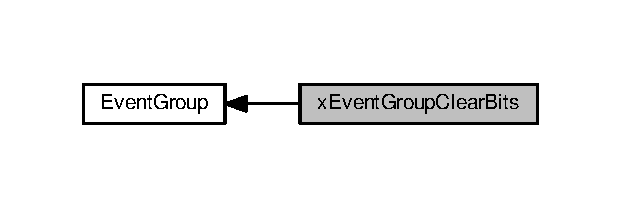
\includegraphics[width=298pt]{d6/dc7/group__xEventGroupClearBits}
\end{center}
\end{figure}
\hyperlink{event__groups_8h}{event\+\_\+groups.\+h} 
\begin{DoxyPre}
   EventBits\_t \hyperlink{event__groups_8h_a0fb72cfdd4f0d5f86d955fc3af448f2a}{xEventGroupClearBits( EventGroupHandle\_t xEventGroup, const EventBits\_t uxBitsToClear )};
\end{DoxyPre}


Clear bits within an event group. This function cannot be called from an interrupt.


\begin{DoxyParams}{Parameters}
{\em x\+Event\+Group} & The event group in which the bits are to be cleared.\\
\hline
{\em ux\+Bits\+To\+Clear} & A bitwise value that indicates the bit or bits to clear in the event group. For example, to clear bit 3 only, set ux\+Bits\+To\+Clear to 0x08. To clear bit 3 and bit 0 set ux\+Bits\+To\+Clear to 0x09.\\
\hline
\end{DoxyParams}
\begin{DoxyReturn}{Returns}
The value of the event group before the specified bits were cleared.
\end{DoxyReturn}
Example usage\+: 
\begin{DoxyPre}
  #define BIT\_0 ( 1 << 0 )
  #define BIT\_4 ( 1 << 4 )\end{DoxyPre}



\begin{DoxyPre}  void aFunction( EventGroupHandle\_t xEventGroup )
  \{
  EventBits\_t uxBits;\end{DoxyPre}



\begin{DoxyPre}    // Clear bit 0 and bit 4 in xEventGroup.
    uxBits = xEventGroupClearBits(
                            xEventGroup,    // The event group being updated.
                            BIT\_0 | BIT\_4 );// The bits being cleared.\end{DoxyPre}



\begin{DoxyPre}    if( ( uxBits \& ( BIT\_0 | BIT\_4 ) ) == ( BIT\_0 | BIT\_4 ) )
    \{
        // Both bit 0 and bit 4 were set before \hyperlink{event__groups_8h_a0fb72cfdd4f0d5f86d955fc3af448f2a}{xEventGroupClearBits()} was
        // called.  Both will now be clear (not set).
    \}
    else if( ( uxBits \& BIT\_0 ) != 0 )
    \{
        // Bit 0 was set before \hyperlink{event__groups_8h_a0fb72cfdd4f0d5f86d955fc3af448f2a}{xEventGroupClearBits()} was called.  It will
        // now be clear.
    \}
    else if( ( uxBits \& BIT\_4 ) != 0 )
    \{
        // Bit 4 was set before \hyperlink{event__groups_8h_a0fb72cfdd4f0d5f86d955fc3af448f2a}{xEventGroupClearBits()} was called.  It will
        // now be clear.
    \}
    else
    \{
        // Neither bit 0 nor bit 4 were set in the first place.
    \}
  \}
  \end{DoxyPre}
 